\documentclass[stu, a4paper, 12pt, floatsintext]{apa7}

% Title Page Stuff
\title{A Design Report for the Transportation Aircraft Designed in Aircraft Systems Design E3 with a Specific Focus on the Design Aspects Covered by the Author.}
\shorttitle{Individual Design Report}
\leftheader{25/03/25}
\authorsnames{Philip Beswick @00662943}
\authorsaffiliations{The University of Salford}
\course{Aircraft Systems Design E3}
\professor{Dr O K Ariff, Dr Andreea Koreanschi}
\duedate{28/03/25}
\abstract{The aircraft designed for this project aims to transport specialty cargo and personnel short distances into areas recently afflicted by natural disasters or warfare. This means that the aircraft has a relatively short Balanced Field length at just over 1000m and a relatively high payload fraction of roughly 30\%. For this project, the author contributed to 3 design aspects in a primary capacity, namely the Initial Weight Estimation, Centre of Gravity Position and Environmental Control Systems. Also, the author contributed in a secondary capacity to Aircraft Drag Prediction, Tailplane and Fin design and Airfield Performance. Generally speaking, the author was tasked with design elements that require a great deal of mathematical analysis, especially when it is being done to verify the design choices that came previously. Overall, the design project was successful as an aircraft was produced that met the team’s design objectives and is competitive with pre-existing aircraft and, of course, is compliant with EASA Part-25 for large Aeroplanes. However, some further tweaking to the airfield performance could be done going forward to make the aircraft even more competitive.}

% Packages Required
\usepackage{csquotes}
\usepackage[english]{babel}
\usepackage[T1]{fontenc}
\usepackage{mathptmx}
\usepackage{multirow}
\usepackage{graphicx}
\usepackage{booktabs}
\usepackage[style=apa,sortcites=true,sorting=nyt,backend=biber]{biblatex}
\usepackage{pgf-pie}
\usepackage{pgfplots}
\usepackage{paracol}
\usepackage{amsmath}
\usepackage{tocloft}
\usepackage{float}
\usepackage{listings}
\usepackage{gensymb}

\addbibresource{bibliography.bib}

\pgfplotsset{compat=1.18}

% Counts chapters numerically
\setcounter{tocdepth}{5}
\setcounter{secnumdepth}{5}

% Counts equations, figures and tables sequentially depending on the chapter
\numberwithin{figure}{section}
\numberwithin{table}{section}
\numberwithin{equation}{section}

\newcommand{\listequationsname}{\Large List of Equations}
\newlistof{myequations}{equ}{\listequationsname}
\newcommand{\myequations}[1]{%
\addcontentsline{equ}{myequations}{\protect\numberline{\theequation}#1}\par}
\setlength{\cftmyequationsnumwidth}{2.5em}% Width of equation number in List of Equations

% Makes sure LaTeX knows where we are :D
\DeclareLanguageMapping{british}{british-apa}

\begin{document}

\maketitle{} % Generates the title page

\tableofcontents

\newpage

\addcontentsline{toc}{subsection}{List of Figures}
\listoffigures
\addcontentsline{toc}{subsection}{List of Tables}
\listoftables
\addcontentsline{toc}{subsection}{List of Equations}
\listofmyequations

%%% Contents of report go here %%%
\newpage

\section{Introduction}
\subsection{Market Survey}
Before the aircraft concept was developed, a thorough market survey was conducted, investigating aircraft that meet the size requirements for this design exercise, which are:
\begin{itemize}
    \item The aircraft must fall into EASA Part-25 (for large aeroplanes, more significant than 5700kg,
    \item The aircraft must seat no more than 24 passengers.     
\end{itemize}
Considering these two characteristics, twenty-three aircraft, a combination of turboprop-powered and jet-powered aircraft, were surveyed in an initial, brief investigation. This initial investigation can be seen in Figure 1.1 (\cite{janes2023}). 

\begin{figure}[H]
    \caption{The initial market survey completed for this design project}
    \label{fig:market_survey_initial}
    \centering
    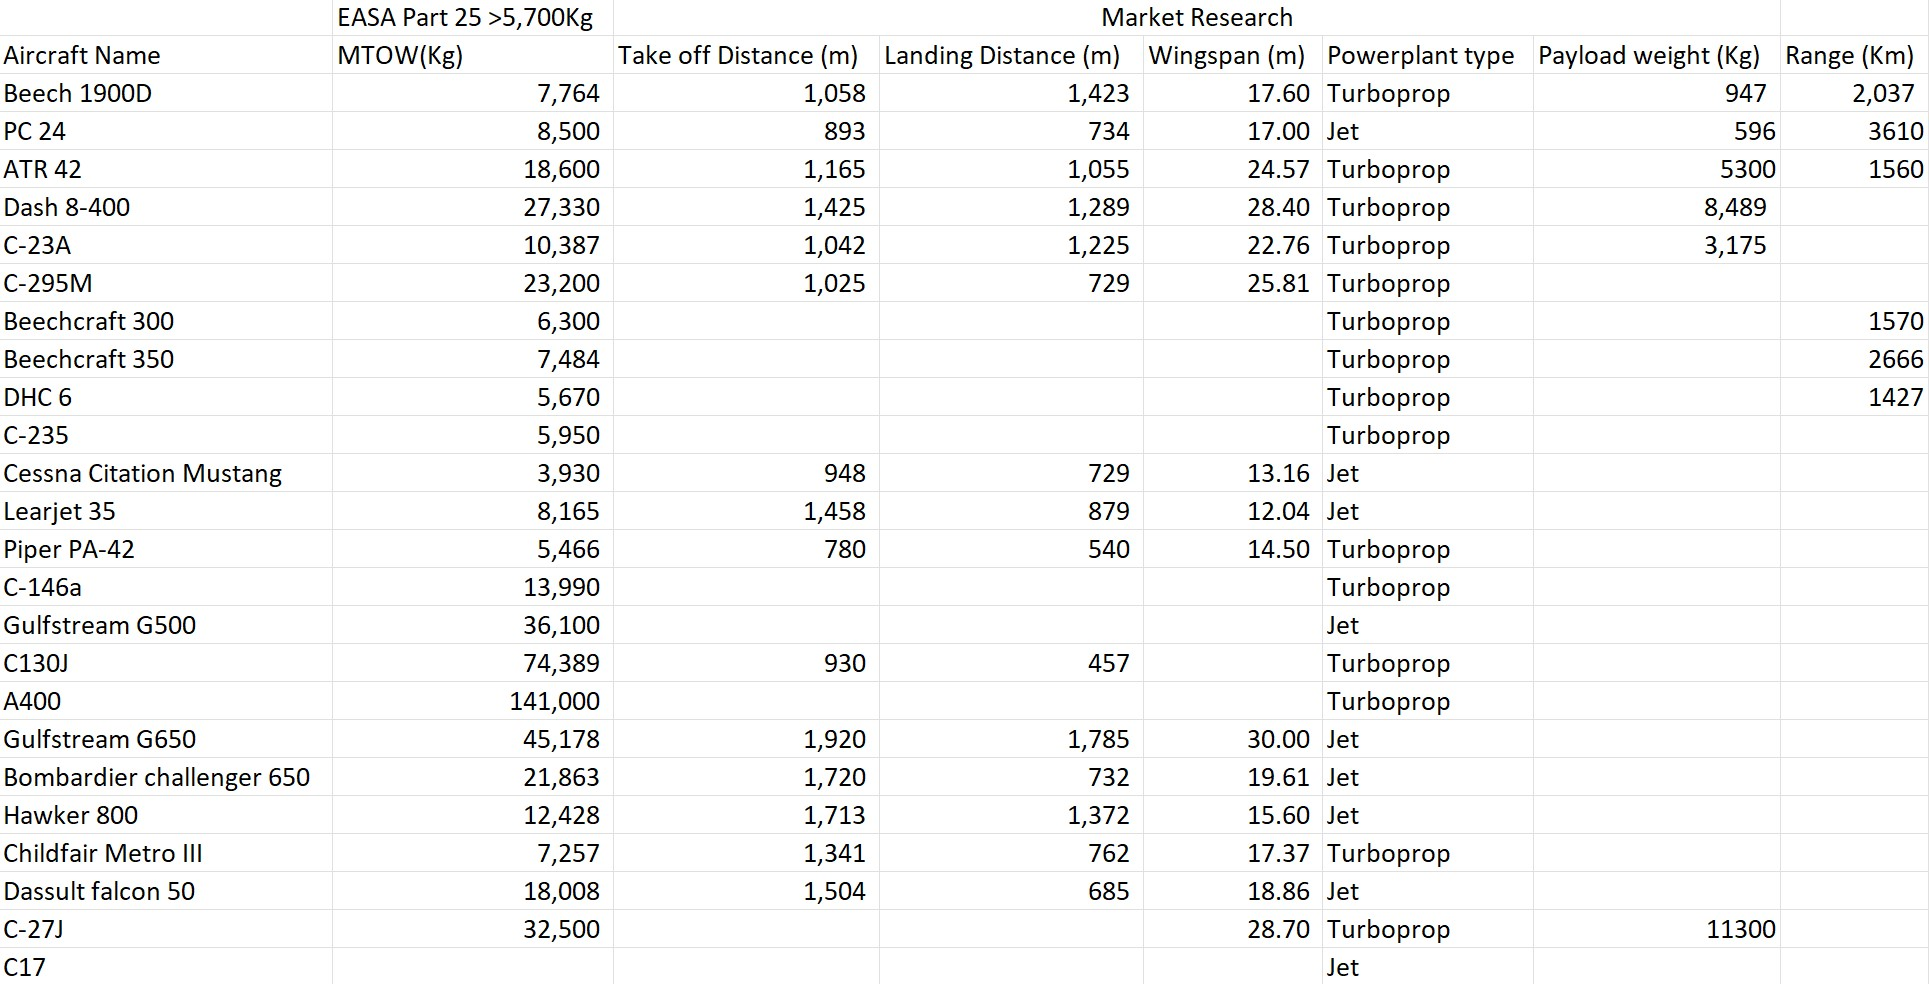
\includegraphics[width=1.1\textwidth]{pictures/market_survey_initial.jpg}
\end{figure}

As seen in Figure 1.1, the scope of the initial investigation was small, but its purpose was twofold:
\begin{enumerate}
    \item To investigate if there is a relationship between aircraft weight and the selected engine type,
    \item To investigate the relationship between aircraft’s airfield performance and weight.
\end{enumerate}

This investigation was successful. From the completed market survey, the design team was able to ascertain that, generally speaking, the lighter aircraft are powered by turboprops rather than jet engines, although exceptions do exist, such as the A400. Additionally, heavier aircraft tended to have worse airfield performance than their lighter counterparts; in this case, worse performance means longer takeoff and landing distances. At this point, the scope of the market survey became narrower but more in-depth, deciding to focus only on ten aircraft, which more closely aligned with a design objective in mind: to transport aid and supplies into disaster zones. Figures 1.2 to 1.5 show the second market survey conducted. 

\begin{figure}[H]
    \caption{The second market survey for the design project - showing general data}
    \label{fig:market_survey_detailed_1}
    \centering
    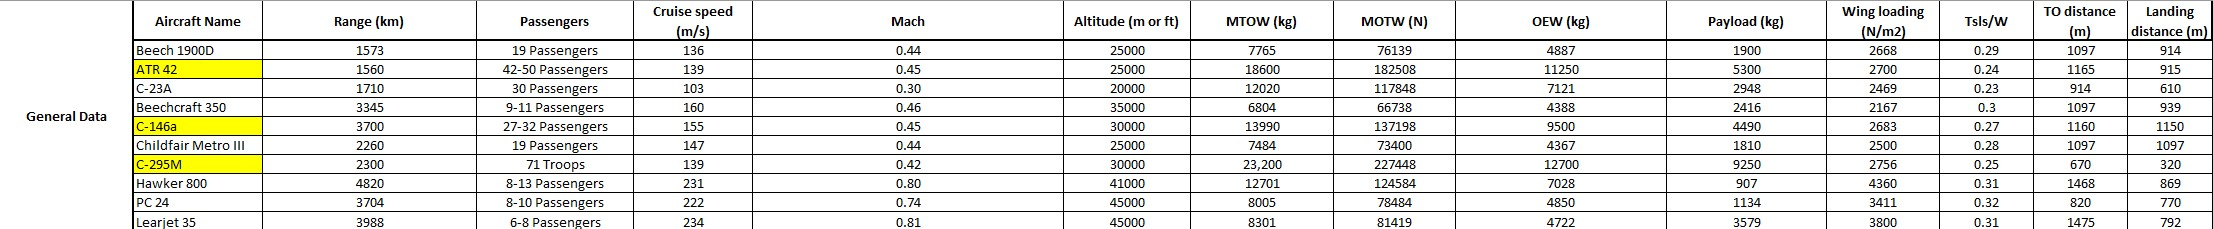
\includegraphics[width=1.1\textwidth]{pictures/market_survey_detailed_1.jpg}
\end{figure}
\begin{figure}[H]
    \caption{The second market survey for the design project - showing engine data}
    \label{fig:market_survey_detailed_2}
    \centering
    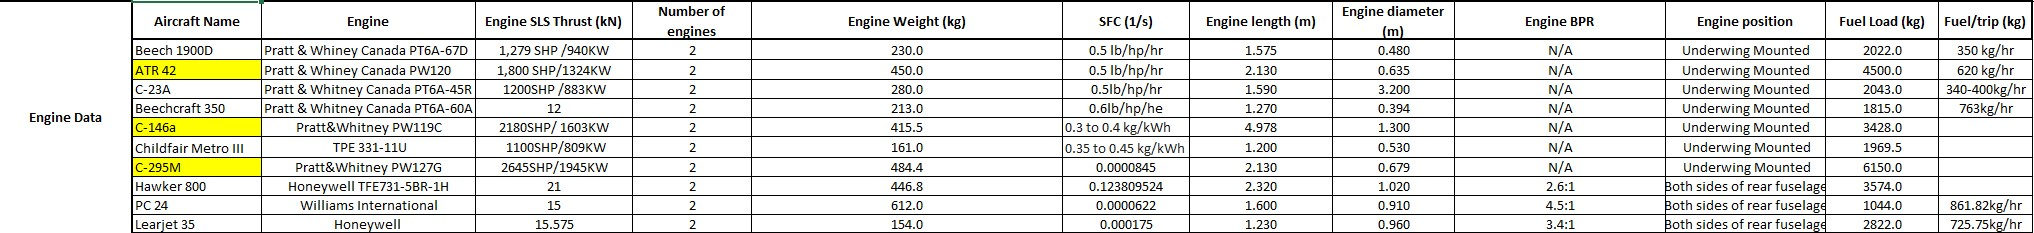
\includegraphics[width=1.1\textwidth]{pictures/market_survey_detailed_2.jpg}
\end{figure}
\begin{figure}[H]
    \caption{The second market survey for the design project - showing dimensions}
    \label{fig:market_survey_detailed_3}
    \centering
    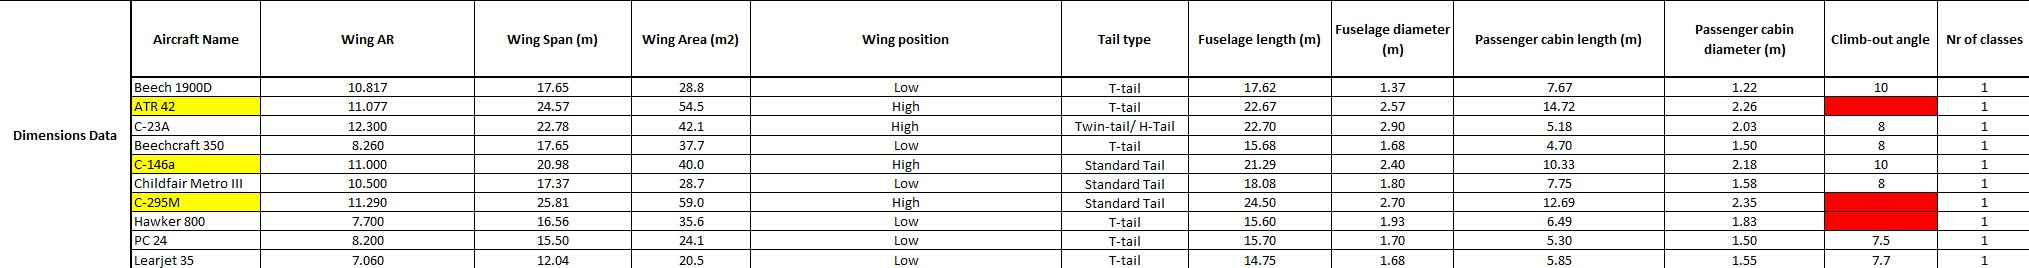
\includegraphics[width=1.1\textwidth]{pictures/market_survey_detailed_3.jpg}
\end{figure}
\begin{figure}[H]
    \caption{The second market survey for the design project - showing weights information}
    \label{fig:market_survey_detailed_4}
    \centering
    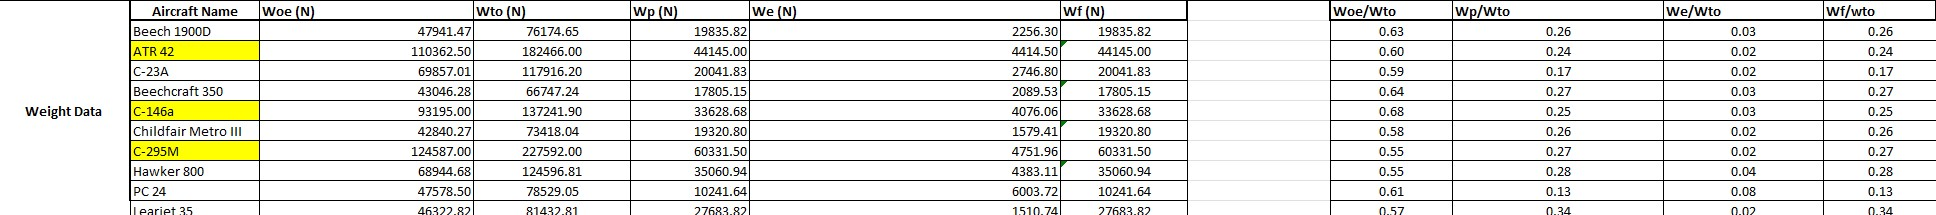
\includegraphics[width=1.1\textwidth]{pictures/market_survey_detailed_4.jpg}
\end{figure}

Figures 1.2 and 1.5 not only confirm the assertions made by the initial market survey but also expand upon them by providing more detailed information. This additional information helps the design team to spot gaps in the existing market; for example, there is no aircraft listed that operates at a short range (less than one thousand kilometers). Furthermore, aircraft such as the ATR-42, which has a very large payload weight (44kN), also has both a very long takeoff distance and landing distance.

This, therefore, became a primary design objective for the group’s aircraft. The goal was to create an aircraft that could transport heavy loads over short distances while also landing and taking off from short, perhaps unconventional airfields.  

\subsection{Design Overview}

The purpose of the aircraft designed in this project is to deliver aid and specialist crew to disaster zones following a natural incident or warfare. The aircraft achieves this by having a short range (one thousand kilometers) but a high payload weight (twenty-four kilo newtons). In addition, the aircraft is capable of taking off from short fields (three hundred and thirty meters long) and landing on fields just over one thousand meters long.  Figure 1.6 shows the plan view of the aircraft.

\begin{figure}[H]
    \caption{The planview of the aircraft designed.}
    \label{fig:aircraft_planview}
    \centering
    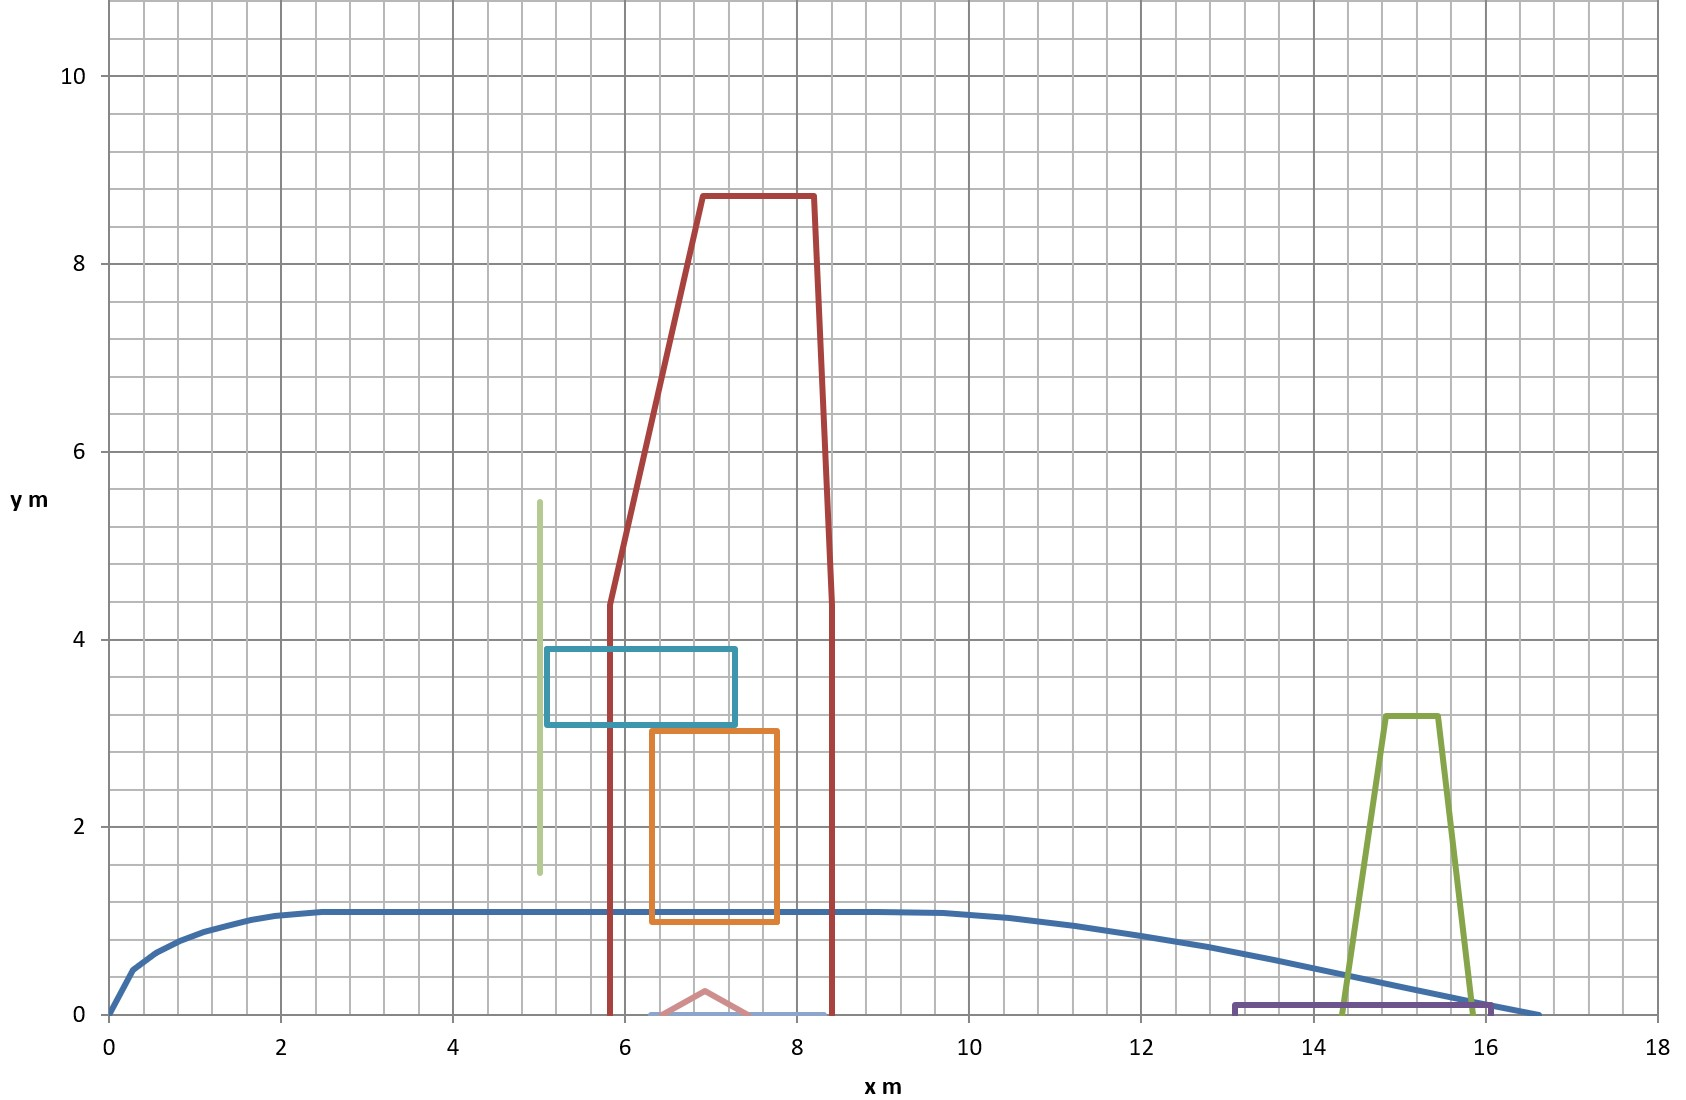
\includegraphics[width=1.1\textwidth]{pictures/planview.jpg}
\end{figure}

The aircraft has a high wing (aspect ratio 9) with engines mounted upon it. In addition, the wing is fitted with both flaps and slats to produce a maximum $C_L$ of 2.3 when taking off, ensuring the aircraft can get off the ground quickly. 

While the aircraft is primarily designed to transport cargo on pallets, the internals of the fuselage are very customisable. If need be, pallet-carrying capabilities can be replaced for people transportation in the event that evacuations are needed following a disaster. When transporting passengers, the aircraft is completely capable of providing a suitable environment onboard, with air mass flow rates exceeding the minimum required by EASA Part-25 in all categories. 

In terms of certification, the aircraft is entirely compliant with EASA Part-25 in all aspects; the aircraft is completely balanced in all loading configurations, and it meets all the necessary requirements when operating with only one engine. For example, it is able to climb out of an airfield at 1.53 $\degree$, when the minimum acceptable climb-out angle is 1.38 $\degree$. 

Finally, the aircraft’s power-to-weight ratio and wing loading is very finely tuned as seen in Figure 1.7.

\begin{figure}[H]
    \caption{The power to weight ratio vs wing laoding of the aircraft.}
    \label{fig:power_to_weight}
    \centering
    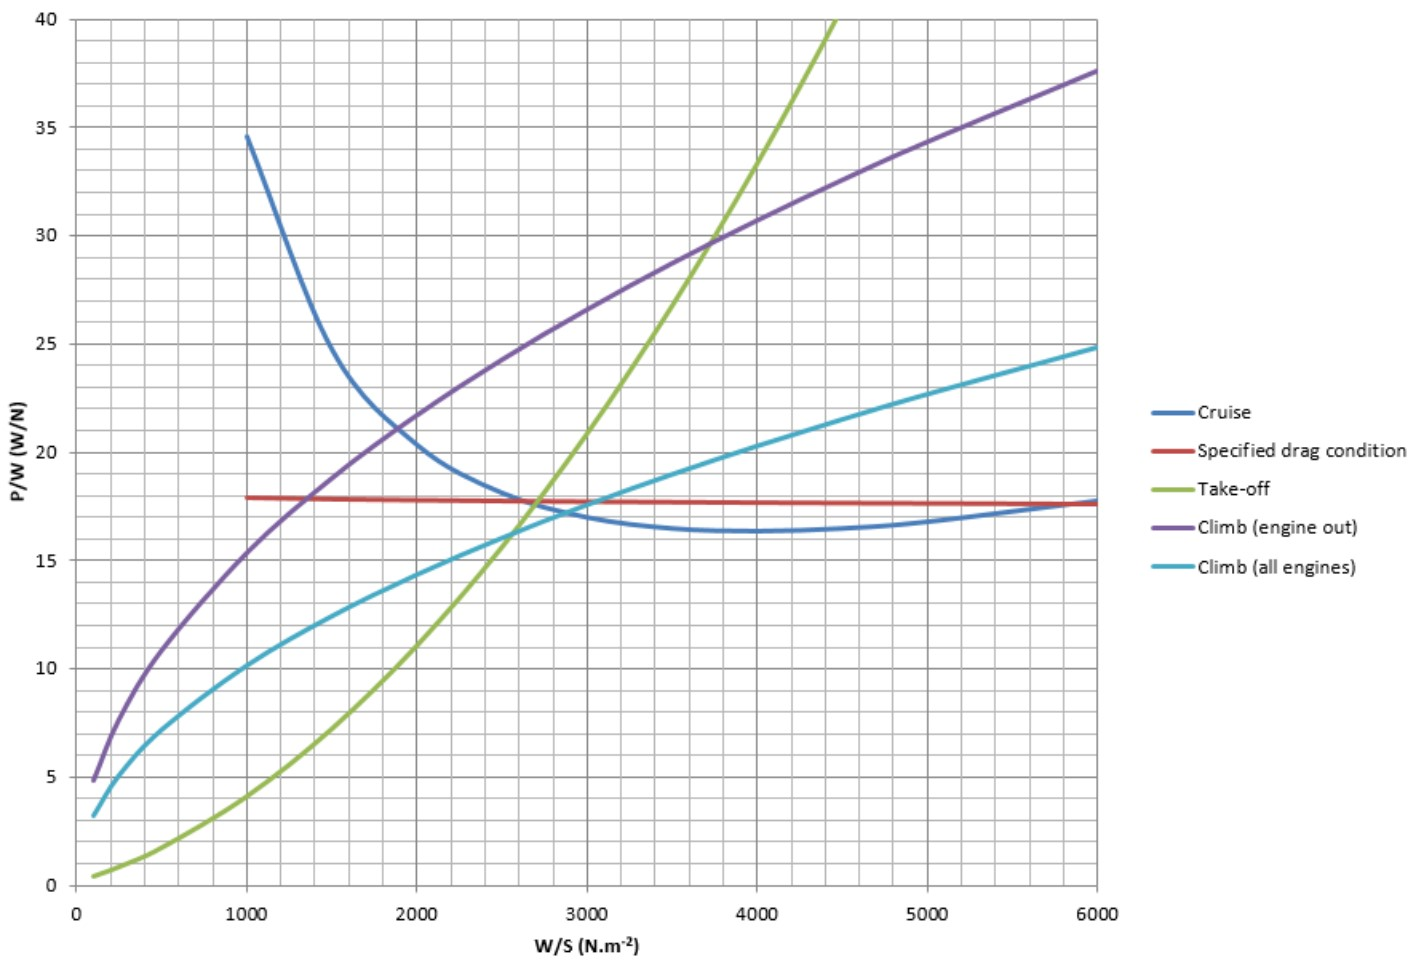
\includegraphics[width=1.1\textwidth]{pictures/power-to-weight.jpg}
\end{figure}

As the lines all intersect at a similar position, the aircraft’s power-to-weight ratio can be confirmed as approximately 17 W/N, with a wing loading of around 2500 $N/m^2$. The fact that the lines all intersect relatively closely provides sufficient evidence that the aircraft will be both aptly powered and stable, with enough lift being generated by the wing.  

Ultimately, the designed aircraft is not only compliant with EASA Part-25, but it is also able to perform its duties as a transport aircraft in very challenging conditions, thanks to its short field operations capabilities and large weight payload.      

\section{Primary Tasks}
The following three tasks, initial weight estimation, centre of gravity and environmental control systems, were all the author's responsibility for this aircraft. As the member of the team with primary responsibility, it was the author’s duty to make the design decisions and justify them with calculations, ensuring that all parameters make both logical sense but also comply with EASA Part-25, the regulatory body that would eventually go on to certify this aircraft.
\subsection{Initial Weight Estimation}
Once the aircraft concept had been completed and unanimously agreed to by the design team, the first task was to estimate the weights. As a reminder, the aircraft was designed to transport specialist cargo, such as medical supplies, and crew into disaster zones. To do this, the aircraft needs to:
\begin{enumerate}
    \item Have a high payload weight fraction and, 
    \item Operate from short, improvised airfields.
\end{enumerate}

Therefore, the aircraft must weigh as little as possible while generating as much lift as possible with its wings. The goal of this element of the design is to tackle the first of those two characteristics. 

It is well known that there is a complex relationship between aircraft range and weight. Logically, two aircraft of identical design will need different amounts of fuel depending on the distance they intend to travel. Therefore, it was quickly decided that aircraft range would not be a factor of primary concern. The aircraft is designed to transport specialty cargo into areas in need of immediate help, and it would be exceptionally useful if help cannot arrive by other methods of transportation such as road, rail or sea. The aircraft only needs to operate relatively short distances to and from a central hub or distribution centre to deliver aid to a local population. 

The following parameters must be known in order to complete the weight estimation:
\begin{enumerate}
    \item Range (km)
    \item Payload (Pax and Cargo)
    \item Power to Weight (P/W) Ratio of the Engine (kW/kN)
    \item Specific Fuel Capacity (SFC) of the Engine ((N/s)/kW)
    \item Wing Aspect Ratio
    \item Fuselage Diameter/Length
    \item Weight per Pax (kg)
\end{enumerate}

Since the aircraft aims to primarily deliver aid supplies rather than transport people, the parameters were slightly modified to account for pallets of cargo that are one cubic meter in size, each capable of carrying 500kg. In addition to the cargo, the aircraft still aims to transport a small number of passengers; this was decided to be seven people maximum.

The parameters related to the engine (P/W and SFC) were taken from known data for the engine selected to power the aircraft, specifically the Pratt and Whitney 127G. The mass of an average person was approximated to be 90kg, and the fuselage D/L was taken to be 0.13. The two parameters not yet discussed, aspect ratio and range, were the most changeable as the design process continued. In total, 10 different initial weight estimations were conducted, with different parameters, to settle on the most acceptable outcome, which will shortly be presented, but the final value for aspect ratio was taken to be 9, and range to be taken at 1000km (it was decided that this would be sufficient to transport supplies short distances into relief areas). Table 3.1 shows the final design values for weight estimation. 

\begin{table}[]
    \centering
    \caption{Final values for weight estimation}
    \label{tab:weight_estimation_table}
    \begin{tabular}{@{}ccccccccc@{}}
    \toprule
    \textbf{Range} & \multicolumn{2}{c}{\textbf{Payload}} & \textbf{P/W} & \textbf{SFC} & \textbf{Aspect Ratio} & \textbf{D/L} & \multicolumn{2}{c}{\textbf{Payload Masses}} \\ \midrule
    km           & Pax             & Pallets            & kW/kN        & (N/s)kW      &                       &              & Pax (kg)           & Pallets (kg)           \\
    1000           & 7               & 4                  & 17.1         & 0.00076      & 9                     & 0.13         & 90                 & 500                    \\ \bottomrule
    \end{tabular}
\end{table}

Before estimating the aircraft’s weight, the fuselage’s length, breadth and depth can be estimated by the following equations, where $x_p$ is the number of passengers and $x_c$ is the number of pallets (or crates): 
\begin{equation}
    Length = 10+0.237x_p + 1.2x_c \, ,
\end{equation}
\myequations{Equation to find the fuselage length.}
\begin{equation}
    Depth = Length \times {{D}\over{L}} \, ,
\end{equation}
\myequations{Equation to find the fuselage depth.}
\begin{equation}
    Breadth = Length \times {{D}\over{L}} \, ,
\end{equation}
\myequations{Equation to find the fuselage breadth.}

With these equations in mind, the fuselage can therefore be estimated, with the results shown in Table 3.2. 

\begin{table}[]
    \centering
    \caption{This table shows the estimated values for the fuselage.}
    \label{tab:fuselage_estimate}
    \begin{tabular}{@{}ccc@{}}
    \toprule
    \textbf{Length (m)} & \textbf{Breadth (m)} & \textbf{Depth (m)} \\ \midrule
    16.62               & 2.2                  & 2.2                \\ \bottomrule
    \end{tabular}
\end{table}

These values can then be used as a basis when the fuselage design is considered later in the design process. The fuel fraction, however, can now be calculated by the following equation: 
\begin{equation}
    ff = 1.046-e^{-0.3504 \times SFC\times {{Range}\over{\sqrt{AR}}}} \, ,
\end{equation}
\myequations{Equation to find the fuel fraction.}

When this equation is applied to the values found in Table 3.1, the fuel fraction obtained is 0.131, rounded to 3 decimal places. This means that roughly 13\% of the aircraft's weight will be taken up by only the fuel needed to fly, assuming maximum takeoff weight. Similarly, the payload weight can be found by the equation:
\begin{equation}
    W_p (N) = g(x_p \times 90 + x_c \times 500 ) \, ,
\end{equation}
\myequations{Equation to find the payload weight.}

Therefore, the payload weight is found to be 24.92kN. Next, the structural weight can be found, which uses the previously defined parameters for fuselage length, breadth and depth. This means that when the fuselage design has been completed, the weights can be re-estimated to find a more precise maximum takeoff weight. Structural weight is found by the following equation:

\begin{equation}
    W_s (N) = 0.15503 \left( L \times {{B \times D}\over{2}} \right)^{1.3909}
\end{equation}
\myequations{Equation to find the structural weight.}

This means that the structural weight was found to be 23.15kN. Finally, the maximum takeoff weight can now be determined by the following equation: 

\begin{equation}
    W_{to} (kN) = {{5+W_p+W_s}\over{0.8-ff}}
\end{equation}

This means that the aircraft's maximum takeoff weight is 84.59kN, which definately falls within the requirements of EASA-Part 25 to be considered a large aeroplane (greater than 5700kg). Ultimately, this is a good design weight for the aircraft as it falls at the lower end of all the aircraft previously discussed in the market survey, while still being able to carry a sufficiently large payload weight. 

\subsection{Centre of Gravity}
Once the aircraft’s wings, fuselage, and weights have been estimated, balancing the centre of gravity is an excellent way to confirm whether the design choices up to that point were suitable. In addition, EASA Part 25 sets out several key parameters in order for the aircraft to be certifiable, most notably that the centre of gravity’s position must be no more than 50\% of the mean aerodynamic chord or less than 25\% of the mean aerodynamic chord. Furthermore, this must be true in both standard and extreme loading conditions to ensure the flight crew can fly the aircraft with relative ease. 

With this in mind, while noting the aircraft’s initial geometry and layout, the centre of gravity positions can be calculated; this was completed using the moment method, with the reference point taken as the aircraft’s nose.  
\begin{equation}
    X_{CG} = \sum \left( {{m_xx}\over{m_{Total}}} \right) \, ,
\end{equation}
\myequations{Equation to find the aircraft's centre of gravity.}
Where $m_x$ is the mass of a specific component and $x$ is the distance of that component from the datum. $m_{Total}$ is the total mass of all components onboard the aircraft.

Table 3.3 shows the values used to calculate $X_{CG}$ assuming maximum fuel and payload. The values given for $m_x$ are as fractions of the aircraft’s maximum takeoff weight.

\begin{table}[H]
    \centering
    \caption{A table showing the weight fraction of all components onboard the aircraft and their respective position relative to the nose of the aircraft. }
    \label{tab:cg_table}
    \begin{tabular}{@{}lll@{}}
    \toprule
    Component          & $m_x$ (Kg)                      & $x$ (m) \\ \midrule
    Wing               & {\color[HTML]{000000} 0.072472} & 7.29    \\
    Fuselage           & 0.17343                         & 6.65    \\
    Tailplane          & 0.01462                         & 15.08   \\
    Fin                & 0.01389                         & 14.35   \\
    Main Undercarriage & 0.03586                         & 8.04    \\
    Nose Undercarriage & 0.01206                         & 2.97    \\
    Flying Controls    & 0.01715                         & 7.11    \\
    Engine Pod         & 0.01833                         & 5.97    \\
    Engine Installed   & 0.10689                         & 5.55    \\
    Airframe           & 0.14                            & 8.31    \\
    Fuel               & 0.13094                         & 7.17    \\
    Payload            & 0.23256                         & 5.84    \\ \bottomrule
    \end{tabular}
\end{table}

Therefore, when applying Equation 3.8, the centre of gravity position is found to be 6.93m from the aircraft’s nose.

At this stage, it's important to consider how some components' mass will change in flight while others will not. For example, the mass of the aircraft's fuel tanks will decrease during the flight as fuel is burned. However, an aircraft's undercarriage will remain at a constant weight throughout the flight. This is an important consideration to make when tweaking component positions in order to gain a suitable $X_{CG}$ position.

Once the position of the centre of gravity is known, relative to the aircraft’s nose, it is vital to find the position of the centre of gravity in terms of the aircraft’s mean aerodynamic chord (MAC). This can be done using the following relationship:

\begin{equation}
    X_{CG_{MAC}} = {{X_{CG}-X_{MAC_{LE}}}\over{MAC}} \, ,
\end{equation}
\myequations{Equation to find the aircraft's centre of gravity as a fraction of MAC.}
Where $X_{MAC_{LE}}$ is the position of the leading edge of the mean aerodynamic chord and $MAC$ is the length of the mean aerodynamic chord. Therefore, the position of the centre of gravity, as a fraction of the mean aerodynamic chord, is given to be 0.31. This value is within the limits that were previously discussed. Yet, this calculation was only completed for one loading condition, maximum fuel capacity and maximum payload. 

To remain completely compliant with EASA Part-25, this process was repeated for several loading conditions, specifically decreasing fuel by 10\% until there was no fuel left for five different payload configurations. The output for these calculations are plotted on the graph shown in Figure 3.1. 

\begin{figure}[H]
    \caption{The change in CG Position as Fuel Load Decreases}
    \label{fig:cg_pos_graph}
    \centering
    \resizebox{1.0\textwidth}{!}{%
    \begin{tikzpicture}
        \begin{axis}[
            title={},
            xlabel={CG Position as \% of MAC},
            ylabel={\% of Fuel load onboard},
            xmin=0.2, xmax=0.55,
            ymin=0, ymax=100,
            xtick={0.2, 0.25, 0.3, 0.35, 0.4, 0.45, 0.5, 0.55},
            ytick={0, 10, 20, 30, 40, 50, 60, 70, 80, 90, 100},
            legend pos=north west,
            ymajorgrids=true,
            grid style=dashed,
        ]
        
        \addplot[
            only marks,
            mark=diamond,
            color=blue,
            ]
            coordinates {
                (0.389, 100)
                (0.386, 90)
                (0.383, 80)
                (0.378, 70)
                (0.373, 60)
                (0.367, 50)
                (0.36, 40)
                (0.35, 30)
                (0.337, 20)
                (0.32, 10)
                (0.294, 0)                                           
            };
        \addplot[
            only marks,
            color=orange,
            mark=square,
            ]
            coordinates {
                (0.4, 100)
                (0.398, 90)
                (0.395, 80)
                (0.392, 70)
                (0.388, 60)
                (0.383, 50)
                (0.377, 40)
                (0.37, 30)
                (0.36, 20)
                (0.346, 10)
                (0.325, 0)                                             
            };
        \addplot[
            only marks,
            color=green,
            mark=triangle,
            ]
            coordinates {
                (0.411, 100)
                (0.41, 90)
                (0.408, 80)
                (0.406, 70)
                (0.403, 60)
                (0.4, 50)
                (0.396, 40)
                (0.391, 30)
                (0.384, 20)
                (0.375, 10)
                (0.36, 0)                                             
            };
        \addplot[
            only marks,
            color=cyan,
            mark=pentagon,
            ]
            coordinates {
                (0.423, 100)
                (0.422, 90)
                (0.421, 80)
                (0.42, 70)
                (0.419, 60)
                (0.418, 50)
                (0.416, 40)
                (0.414, 30)
                (0.411, 20)
                (0.406, 10)
                (0.399, 0)                                              
            };
        \addplot[
            only marks,
            color=black,
            mark=+,
            ]
            coordinates {
                (0.434, 100)
                (0.435, 90)
                (0.435, 80)
                (0.435, 70)
                (0.436, 60)
                (0.437, 50)
                (0.437, 40)
                (0.438, 30)
                (0.44, 20)
                (0.441, 10)
                (0.445, 0)                                             
            };
            \addplot[
                only marks,
                color=brown,
                mark=star,
                ]
                coordinates {
                    (0.447, 100)
                    (0.448, 90)
                    (0.45, 80)
                    (0.451, 70)
                    (0.454, 60)
                    (0.456, 50)
                    (0.46, 40)
                    (0.465, 30)
                    (0.471, 20)
                    (0.481, 10)
                    (0.496, 0)                                                      
                };
            \addplot[
                color=red,
                mark=circle,
                ]
                coordinates {
                    (0.25, 100)
                    (0.25, 90)
                    (0.25, 80)
                    (0.25, 70)
                    (0.25, 60)
                    (0.25, 50)
                    (0.25, 40)
                    (0.25, 30)
                    (0.25, 20)
                    (0.25, 10)
                    (0.25, 0)                                                   
                };
            \addplot[
                color=red,
                mark=circle,
                ]
                coordinates {
                    (0.5, 100)
                    (0.5, 90)
                    (0.5, 80)
                    (0.5, 70)
                    (0.5, 60)
                    (0.5, 50)
                    (0.5, 40)
                    (0.5, 30)
                    (0.5, 20)
                    (0.5, 10)
                    (0.5, 0)                                                    
                };
            \legend{100\% Payload, 80\% Payload, 60\%Payload, 40\% Payload, 20\% Payload, 0\% Payload}
        \end{axis}
    \end{tikzpicture}
    }
\end{figure}

Figure 3.1 ultimately shows that no matter the aircraft's loading configuration, the CG position remains within the acceptable limits imposed in EASA Part-25. This means that the aircraft has been successfully balanced and that the initial aircraft configuration is acceptable and can be built on in further elements, such as the design of the tailplane and undercarriage. 

Throughout the design process, the CG was constantly tweaked. For example, after completing the fin and tailplane design, more accurate values for tailplane weight and position could be used and implemented in the CG balancing method. This meant that the overall aircraft balancing was constantly being tweaked by slightly moving components with constant weight throughout the flight. The values discussed in this report represent the final values once the design had been completed.  

\subsection{Environmental Control Systems}
Environmental Control systems are crucial to ensure that passengers remain not only comfortable but alive during extended periods at high altitudes. Of course, the aircraft that is being designed is primarily for the transportation of equipment and supplies, but even then, they must be kept at a regulated temperature to ensure that they are free from damage when ready for use. While EASA does not have any particular requirements for environmental control systems, most modern aircraft maintain approximately 10 cubic feet per minute per passenger. This will be a design goal that is kept in mind throughout this process. 

The following two subsections are dedicated to evaluating the fuselage’s skin temperature in various conditions so that heat loading can be calculated for the aircraft in those same conditions. 
\subsubsection{Airfield Condition}
When aircraft are on the ground at an airfield, the cabin temperature will be maintained to create a comfortable environment. For the purposes of these calculations, two extreme conditions will be considered: a hot day ($45 \degree$) without wind and a cold day ($-20 \degree$) without wind. These two conditions will see the environmental control systems work at their hardest, as in the presence of wind, some natural cooling will occur due to decreased fuselage skin temperature. The following parameters are used in this set of calculations:
\begin{table}[]
    \centering
    \caption{This table shows the parameters used when calculating the skin temperature on hot and cold days}
    \label{tab:ecs_airfield_parameters}
    \begin{tabular}{@{}cc@{}}
    \toprule
    Skin Temperature          & $T_s$ \\ 
    Cabin Temperature         & $T_c$ \\
    Ambient Temperature       & $T_1$ \\
    Heat Transfer Coefficient & $U_f$ \\ \bottomrule
    \end{tabular}
\end{table}
These parameters are then applied to Equations 3.10 and 3.11 for a cold and hot day, respectively, where $U_f$ takes the value of 2.44. 
\begin{equation}
    1.25(T_s-T_1)^{1.33} + U_f(T_s-T_c) = 0 \, ,
\end{equation}
\myequations{Airfield Condition - Cold Day Equation to find $T_s$}
\begin{equation}
    1.25(T_s-T_1)^{1.33} + U_f(T_s-T_c) = 90 \, ,
\end{equation}
\myequations{Airfield Condition - Hot Day Equation to find $T_s$}

On both days, the objective is to solve the equations for $T_s$ by iteration so that the left-hand side is approximately equal to their respective values. After much mathematics, it was found that on a hot day, the value of $T_s$ is roughly equal to $50.2905\degree C$ and on a cold day, the value of $T_s$ is approximately $-1.439\degree C$. An example of these iterative calculations can be seen in in Figures 3.2 (hot day) and Figures 3.3 (cold day).

\begin{figure}[H]
    \caption{The iterative process used to find the value of $T_s$ on a hot day, in airfield condition.}
    \label{fig:ecs_hot}
    \centering
    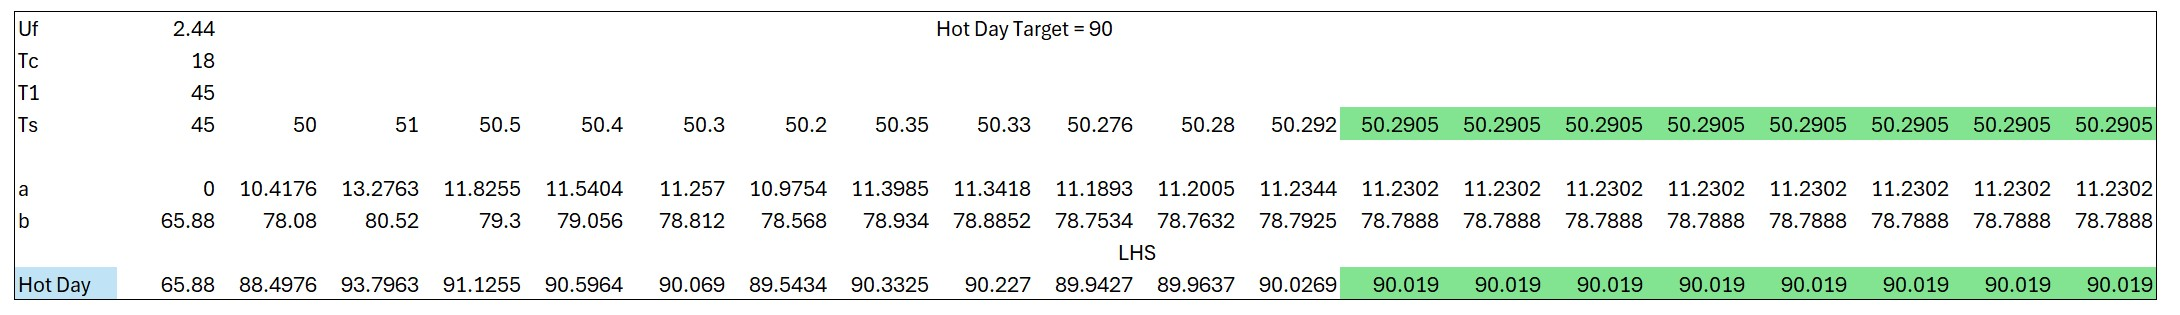
\includegraphics[width=1.1\textwidth]{pictures/ECS_hot_iteration.jpg}
\end{figure}

\begin{figure}[H]
    \caption{The iterative process used to find the value of $T_s$ on a cold day, in airfield condition.}
    \label{fig:ecs_cold}
    \centering
    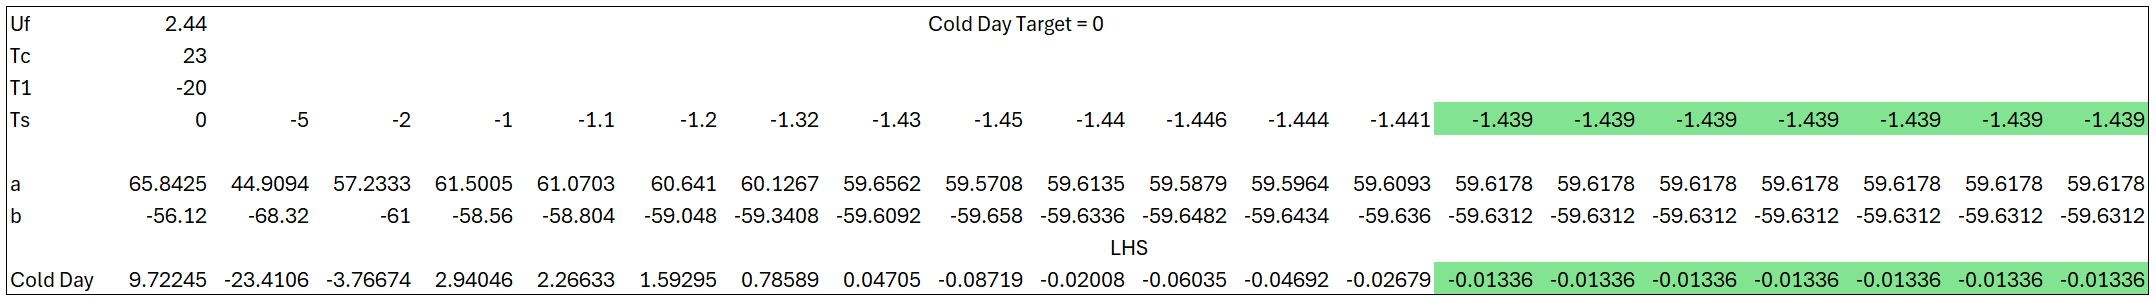
\includegraphics[width=1.1\textwidth]{pictures/ECS_cold_iteration.jpg}
\end{figure}

\subsubsection{Inflight Condition}
When calculating a value for $T_s$ in flight, the mathematical approach is much simpler, as no iterative processes are needed, unlike in the airfield condition. However, it is much more calculation heavy, as the skin temperature will depend on both the aircraft’s cruising speed and altitude. In flight, the heat transfer through the cabin walls is convected to flow around the aircraft. The mathematical expression for this involves Reynold’s analogy between heat transfer and skin friction, which is expressed in terms of the Stanton Number, $S_t$, as seen in Equation 3.12.  
\begin{equation}
    S_t = {{q}\over{\rho u C_p (T_r-T_s)}} \, ,
\end{equation}
\myequations{Equation for Stanton Number $T_s$.}

Where $q$ is equal to the heat transfer per unit area of skin and $T_r$ is the recovery temperature of the skin surface. The equation for $T_r$ is seen in Equation 3.13. In addition, $q$ can be expressed by Equation 3.14, where $S_f$ is the fuselage surface area where heat transfer takes place.

\begin{equation}
    T_r = T_1 (1+0.18M^2) \, ,
\end{equation}
\myequations{The equation for the recovery temperature $T_r$.}
\begin{equation}
    q = {{Q}\over{S_f}} = U_f(T_s-T_c) \, ,
\end{equation}
\myequations{The equation for the heat transfer per unit area of skin $q$.}

This means that an equation for $T_s$ can be constructed, assuming that the Stanton number can be evaluated differently. This is the case, as the Stanton number can be found using the relationship between the average skin friction coefficient ($C_F$) and the Prandtl number ($\sigma$), which is normally taken as 0.72 in air, and is shown in Equation 3.15.

\begin{equation}
    S_t = {{C_F}\over{2\sigma ^{{2}\over{3}}}} \, ,
\end{equation}
\myequations{The equation for the Stanton Number in terms of $C_F$ and $\sigma$.}

The average skin friction coefficient can be found using the Prandtl-Schlichting relationship (Equation 3.17), using the Reynold's number based on fuselage length ($R_L$), which is given by Equation 3.16.

\begin{equation}
    R_L = {{\rho uL}\over{\mu}} \, ,
\end{equation}
\myequations{Equation based for the Reynolds number based on the Fuselage length.}
\begin{equation}
    C_F = 0.455(1-0.1M)(log_{10}R_L)^{-2.58} \, ,
\end{equation}
Finally, this means that the equation for $T_s$ in terms of the Stanton Number can be constructed, as shown in Equation 3.18.

\begin{equation}
    T_S = {{S_t \rho u C_p T_r + U_f T_c}\over{U_f + S_t \rho u C_p}} \, ,
\end{equation}

Therefore, considering a cruising speed of 140 meters per second and a fuselage length of 16.62 meters, $C_F$ can be calculated using Equation 3.17 and a value of 0.002143 is obtained. This means that the Stanton Number can be evaluated using Equation 3.15, and a value of 0.001334 is obtained. At a cruising altitude of twenty thousand feet, the ambient temperature is approximately -27.1$\degree C$, therefore, using Equation 3.13, the recovery temperature is found to be -28.05$\degree C$. Finally, this means that the skin temperature can be obtained using Equation 3.18, assuming the value of $T_c$ is cool at approximately 18$\degree C$, the value of the skin temperature is -27.06$\degree C$.  

\subsubsection{Calculating Heat Load}

Now that the skin temperature values have been obtained in the three different conditions, the heat load of the Environmental Control system can be calculated for each. Heat loading, $Q$, is given by Equation 3.19, where $N_p$ is the number of passengers (7), ${{D}\over{L}}
$ is the drag to lift ratio, ${{W_p}\over{W}}$ is the payload weight to weight ratio, and V is the cruise speed. 

\begin{equation}
    Q = U_f S_f (T_s-T_c) + 450 \times 2.2 + 4.75N_p(39.8-T_c) + 0.001 {{D}\over{L}}{{W_p}\over{W}}VW_p \, ,
\end{equation}

Table 3.5 shows the various heat loads and their respective skin temperatures.

\begin{table}[H]
    \centering
    \caption{This table shows the heat loads for different skin temperatures and conditions}
    \label{tab:ecs_final}
    \begin{tabular}{@{}ccc@{}}
    \toprule
    \textbf{Skin Temperature $T_s$ ($\degree C$)} & \textbf{Heat Load Q (W)} & \textbf{Condition} \\ \midrule
    -1.44                                        & -5151.02                 & Airfield Cold      \\
    50.29                                        & 11943.91                 & Airfield Hot       \\
    -27.06                                       & -11170.12                & Cruising           \\ \bottomrule
    \end{tabular}
\end{table}

With the values of heat loading known, the mass flow rate for both the environmental control system ($\dot m_{ecs}$) and the recirculation system ($\dot m_r$) can be obtained by Equations 3.20 and  3.21, respectively. 

\begin{equation}
    \dot m_{ecs} = {{Q}\over{C_p(T_c-T_{ecs})}} \, ,
\end{equation}
\myequations{The equation to find $\dot m_{ecs}$.}
\begin{equation}
    \dot m_{r} = {{T_{in}\dot m_{ecs}-\dot m_{ecs}T_{ecs}}\over{T_c-T_{in}}} \, ,
\end{equation}
\myequations{The equation to find $\dot m_{r}$.}

Table 3.6 shows the various mass flow rates, for each of the 3 conditions. 

\begin{table}[H]
    \centering
    \caption{This table shows the different mass flow rates in different conditions. }
    \label{tab:ecs_final_mass}
    \begin{tabular}{@{}ccc@{}}
    \toprule
    \textbf{$\dot m_{ecs}$ (kg/s)} & \textbf{$\dot m_r$ (kg/s)} & \textbf{Condition} \\ \midrule
    0.109                          & 0.025                      & Airfield Cold      \\
    0.914                          & 0.552                      & Airfield Hot       \\
    0.236                          & 0.047                      & Cruising           \\ \bottomrule
    \end{tabular}
\end{table}

These values are acceptable for the heat loading of the aircraft’s environmental control system, and the values for mass flow rate are acceptable, enough air is being provided to the cabin in all phases of flight, and the percentage of air being recirculated is less than 45\% in all conditions, thus meeting the necessary certifcation requirements apart of EASA Part-25. 

\section{Secondary Tasks}
The following tasks, aircraft drag prediction, tail and fin design and airfield performance, were assigned to the author in a secondary capacity. This means that it was the author’s duty to confirm and corroborate the primary’s decisions by repeating calculations to ensure that their decisions made sense and met the necessary certification requirements outlined in EASA Part-25.  
\subsection{Aircraft Drag Prediction}
When mathematically predicting the drag of the aircraft, the drag area methods are employed to find the drag induced by:
\begin{enumerate}
    \item The wing,
    \item The fuselage,
    \item The nacelles.
\end{enumerate}
In order to complete these calculations, a number of parameters are needed; these can be found in Table 4.1. 
\begin{table}[H]
    \centering
    \caption{Table of values used to compute drag prediction at cruising altitude.}
    \label{tab:drag_cruise_table}
    \begin{tabular}{@{}lll@{}}
    \toprule
    \multicolumn{1}{c}{\textbf{Parameter}} & \multicolumn{1}{c}{\textbf{Mathematical Symbol}} & \multicolumn{1}{c}{\textbf{Value for our Aircraft}} \\ \midrule
    Airpseed                               & $V$                                              & 140                                                 \\
    Altitude                               & $h$                                              & 7.62                                                \\
    Wing Area                              & $S$                                              & 33.836                                              \\
    Thickness to Chord Ratio               & $t_c$                                              & 0.18                                                \\
    Quarter Chord Sweep                    & $\Lambda_{{{1}\over{4}}}$                         & 5                                                   \\
    Fuselage Length                        & $l_f$                                            & 16.62                                               \\
    Fuselage Breadth                       & $b_f$                                            & 2.2                                                 \\
    Fuselage Depth                         & $d_f$                                            & 2.2                                                 \\
    Number of Engines                      & $n_e$                                            & 2                                                   \\
    Engine Power                           & $P$                                              & 1945                                                \\
    Engine $k_i$                           & $k_i$                                            & 1                                                   \\
    Maximum Takeoff Weight                 & $W_{TO}$                                         & 8.6                                                 \\
    Empennage Factor                       & $C_e$                                            & 1.24                                                \\
    Undercarraige Factor                   & $C_{UC}$                                         & 1.08                                                \\
    Compressibility Increment              & $c$                                              & 0.0005                                              \\
    Drag induced by flaps at takeoff       & $\Delta C_{Dof}$                                 & 0.03156                                             \\
    Drag induced by flaps at landing       & $\Delta C_{Dla}$                                 & 0.033708                                            \\ \bottomrule
    \end{tabular}
\end{table}

It is important to remember the fact that these values would calculate drag at cruising speed only. By modifying the values for airspeed and altitude, drag could be predicted in different phases of flight. This will be completed, and the different values used for airspeed and altitude will be shown in Table 4.2.

\begin{table}[H]
    \centering
    \caption{The different values of airspeed and altitude used to compute drag in different phases of flight.}
    \label{tab:drag_pred_phase_table}
    \begin{tabular}{@{}c c c @{}}
    \toprule
    \textbf{Condition} & \textbf{Altitude (km)} & \textbf{Airspeed (m/s)} \\ \midrule
    \textbf{2000ft}    & 0.6096                 & 82                      \\
    \textbf{Gear Down} & 0.6096                 & 77                      \\
    \textbf{Landing}   & 0.3048                 & 72                      \\
    \textbf{Takeoff}   & 0.3048                 & 72                      \\ \bottomrule
    \end{tabular}
\end{table}

Equations 4.1 (wing drag area), 4.2 (fuselage drag area), 4.3 (nacelle drag area)  show how the different drag areas can be calculated based on the parameters detailed in Table 4.1, whereas Equation 4.4 shows how to find the overall drag area of the aircraft.

\begin{equation}
    (C_DS)_w = 0.0054(1+3t_c\times cos^2(\Lambda_{{1}\over{4}})) \, ,
\end{equation}
\myequations{The equation to find the wing drag area.}
\begin{equation}
    (C_DS)_f = 0.0031l_f(b_f+d_f) \, ,
\end{equation}
\myequations{The equation to find the fuselage drag area.}
\begin{equation}
    (C_DS)_p = 0.1k_i{{P}\over{717.2P^{0.168}}}n_e \, ,
\end{equation}
\myequations{The equation to find the nacelle drag area.}
\begin{equation}
    C_DS = (47Re^{-0.2})C_{UC}(C_e((C_DS)_w+(C_DS)_f)+(C_DS)_p) \, ,
\end{equation}
\myequations{The equation to find the overall drag area.}
Once these equations have been applied to the values previously discussed in Tables 4.1 and 4.2, values for the coefficients of drag can be calculated, the Equation for clean drag ($C_{DO}$) can be seen in Equation 4.5, the equation for drag due to undercarriage deployment ($(C_{DO})_{uc}$) can be seein in Equation 4.6 and finally drag due to flap extension at takeoff ($(C_{DO})_{to}$) and landing ($(C_{DO})_{la}$) can be seen in Equations 4.7 and 4.8 respectively. 
\begin{equation}
    C_{DO}= {{C_DS}\over{S}} + c \, ,
\end{equation}
\myequations{The equation to find the clean drag coefficient.}
\begin{equation}
    (C_{DO})_{uc}= (0.095+1*0.063) \left( {{W_{TO}^{0.785}}\over{S}} \right) \, ,
\end{equation}
\myequations{The equation to find the drag coefficient incuded by undercarriage deployment.}
\begin{equation}
    (C_{DO})_{to}= C_{DO}+(C_{DO})_{uc}+ \Delta C_{Dof}\, ,
\end{equation}
\myequations{The equation to find the drag coefficient incuded by flaps during takeoff.}
\begin{equation}
    (C_{DO})_{la}= C_{DO}+(C_{DO})_{uc}+ \Delta C_{Dla}\, ,
\end{equation}
\myequations{The equation to find the drag coefficient incuded by flaps during landing.}

Now that all the equations have been defined, the coefficient of drag can be calculated in many different conditions, the results of which are shown in Table 4.3. 

\begin{table}[]
    \centering
    \caption{The table shows the different drag coefficients at five different phases of flight.}
    \label{tab:drag_values}
    \begin{tabular}{@{}cccccc@{}}
    \toprule 
    \textbf{Condition}        & \textbf{Altitude (km)} & \textbf{Airspeed} & \textbf{Gear} & \textbf{Flaps} & \textbf{Drag} \\ \midrule
    \textbf{Cruise (25000ft)} & 7.62                   & 140               & No            & No             & 0.03109       \\ 
    \textbf{2000ft}           & 0.6096                 & 82                & No            & No             & 0.030617      \\
    \textbf{Gear Down}        & 0.6096                 & 77                & Yes           & 15             & 0.089991      \\
    \textbf{Landing}          & 0.3048                 & 72                & Yes           & 45             & 0.090253      \\ 
    \textbf{Takeoff}          & 0.3048                 & 72                & Yes           & 30             & 0.088105      \\ \bottomrule
    \end{tabular}
\end{table}

These values are sufficiently close to those calculated by the primary designer for the aircraft drag prediction. This process cannot comment on the choices made by the primary designer as this element of the design process is purely analytical, which attempts to identify if the aircraft performs with an acceptable drag component. However, this process can reasonably say that the primary designer performed the calculations correctly and to a high degree of accuracy as the values obtained by the independent methods are within a reasonable degree of accuracy of one another.   
\subsection{Tailplane and Fin Design}
\subsubsection{Tailplane Design}
Before the sizing of the fin can be completed, the tailplane first must be sized and appropriately positioned on the fuselage to give a balanced aircraft. The following parameters were chosen for the tailplane, they can be seen in Table 4.4. 

\begin{table}[H]
    \centering
    \caption{This table shows the design characteristics of the aircraft's tailplane. }
    \label{tab:tailplane_table}
    \begin{tabular}{@{}cc@{}}
    \toprule
    \textbf{Parameter}         & \textbf{Value} \\ \midrule
    Aspect Ratio               & 5              \\
    Tail Moment Arm (m)        & 10.9           \\
    Tailplane Sweep ($\degree$) & 5              \\ \bottomrule
    \end{tabular}
\end{table}

A numerical analysis is done on this data and the aircraft’s general design information to create Figure 4.1. This graph shows how stable the aircraft is with the addition of the tailplane, taking into account the centre of gravity’s position range. This graph not only shows that the CG positions fall within the forward and aft locus for the tailplane to be balanced. Additionally, the aircraft will be easily controllable in severe phases of flight, such as stalls or harsh manoeuvres, since their plots also lie within the CG lower and maximum boundaries. 

\begin{figure}[H]
    \caption{The graphical tailplane analysis conducted to ensure it balances the aircraft correctly.}
    \label{fig:tailplane}
    \centering
    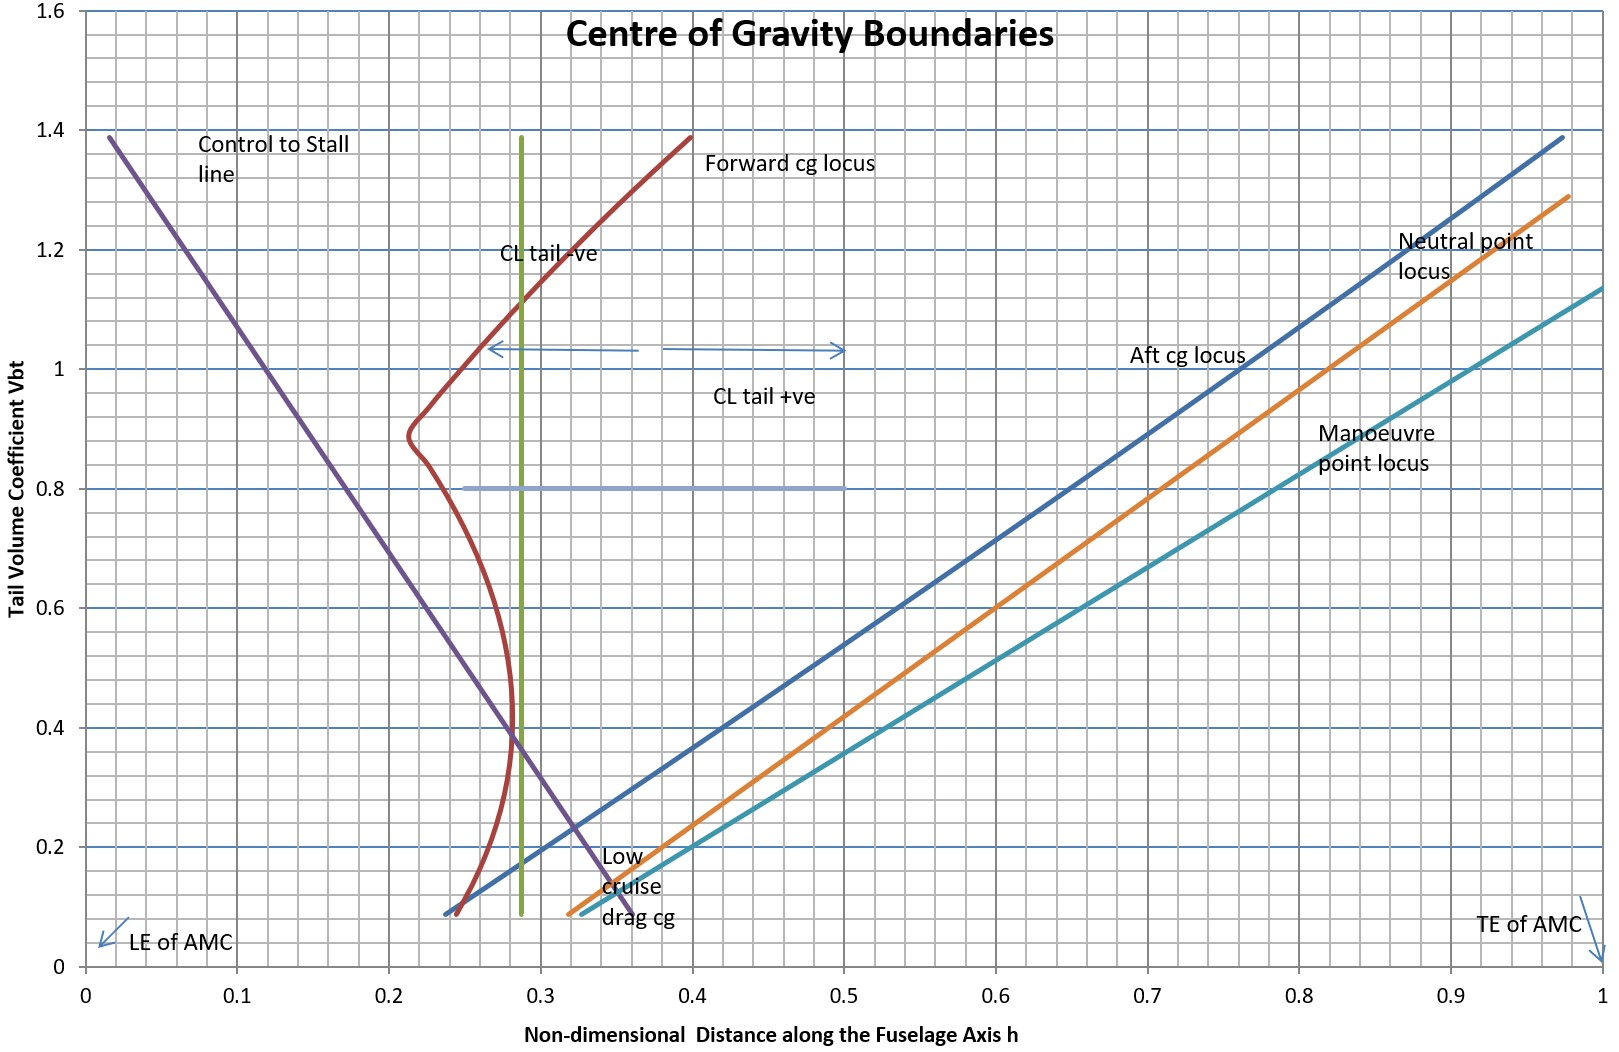
\includegraphics[width=1.1\textwidth]{pictures/tailplane_analysis.jpg}
\end{figure}

The graphical analysis of the tailplane design confirms that the primary designer chose good design parameters (as seen in Table 4.4) for the tailplane. Furthermore, the graphical analysis performed by the primary and secondary designers yielded very similar results, and therefore, there is a high level of confidence that the completed analysis shows a true reflection of the tailplane’s impact on the aircraft’s balance.

\subsubsection{Fin Design}

Now that the tailplane has been sized and appropriately placed on the fuselage, the vertical fin can be designed. The primary designer selected the parameters seen in Table 4.5. 

\begin{table}[H]
    \centering
    \caption{This table shows the design characteristics of the aircraft's fin. }
    \label{tab:fin_table}
    \begin{tabular}{@{}cc@{}}
    \toprule
    \textbf{Parameter}       & \textbf{Value} \\ \midrule
    Aspect Ratio (Fin)       & 2.5            \\
    Aspect Ratio (Rudder)    & 2.5            \\
    Rudder Sweep ($\degree$) & 40             \\ \bottomrule
    \end{tabular}
\end{table}
    
From these parameters and other aircraft data, the fin volume coefficient ($V_{bf}$) can be obtained by Equation 4.9. 

\begin{equation}
    V_{bf} = k_e \left\{ \left[ \frac{\left(\frac{P}{W}\right)}{n_e} \right] \left( \frac{y_e}{b} \right) C_{L_{\max}} \right\} \frac{S_f}{S_{fr}} \Bigg/ \left\{ \left( 1 - \frac{W_p}{W} \right) \left( \frac{S_r}{S_{fr}} AR_{fr} \cos\Lambda_r \right)^{\frac{1}{3}} \right\} /, ,
\end{equation}
\myequations{The equation for Fin Volume Coefficient.}
Application of this equation results in a value of $V_bf$ of 0.32097. This is slightly higher than most conventional fins, most fins have a value between 0.05 and 0.25. However, this is to be expected as a slightly larger fin was chosen so that the fin contributes as much lift as possible while minimising the drag produced by the turboprobs mounted on the wing.   

The analysis produced by both secondary and primary yeilded similar results and therefore it can be said with, a high degree of confidence, that the impact of the fin's sizing has been fully understood and accounted for by the design team.
\subsection{Airfield Performance}
Similarly to Chapter 4.1, when assessing airfield performance in the role of a secondary, the goal is to not comment on design choices made as no unique decisions are made at this phase of design. Instead, the performance of the aircraft is estimated based on its design values by a numerical analysis. The goal of said analysis is to obtain values for:
\begin{enumerate}
    \item Aircraft Landing distance, in meters, 
    \item Aircraft takeoff distance, in meters,
    \item Aircraft climb out angle, in degrees, for an all engine case and an engine failure case.
\end{enumerate}

Furthermore, it is important that these parameters comply with EASA Part-25 regulations for airfield performance. In particular, EASA states that in an engine failure situation, the minimum climb out angle for a large aeroplane is 1.38 $\degree$. This design phase is the final checkpoint for the aircraft designed for this project and will ultimately inform the design team if the design objectives have been met. After some mathematical analysis, the takeoff speed for the aircraft is found to be 44m/s and is found by Equation 4.10. 
\begin{equation}
    V_{TO} = \sqrt{{{2W/S}\over{\rho (C_L)_{max}}}} \, ,
\end{equation}
\myequations{Equation to find takeoff speed of the aircraft.}
Also, the takeoff field length is found to be 339m, with an abort takeoff distance of 204m. This means that the speed for $V_1$ will be set so that there is always a minimum distance of 204m so that the aircraft can stop safely. In the event of an engine failure past the point of $V_1$, the takeoff distance will naturally increase, in this case to a distance of 892m, which takes the value of the Balanced Field Length. This is the minimum safe distance that an aircraft can take off at as there should always be preparations for an aborted takeoff or engine failure past the point of no return. These values are sufficiently close to those calculated by the primary designer at this stage, and therefore, there is a high level of confidence that they are the true, correct values for the aircraft.

mportantly, the climb-out angle for the aircraft was also calculated, both for an engine failure and for normal takeoff conditions. In normal takeoff conditions, the climb out angle was calculated to be 12 $\degree$, whereas in an engine failure condition, the climb out angle was found to be 1.53 $\degree$. Importantly, these values are both sufficiently close to those calculated by the primary designer but also completely comply with EASA Part-25 requirements for large aeroplanes.

Finally, the landing distance, with included factor of safety, was found to be 1005m. Again, this value is sufficiently close to the one calculated by the primary designer.

There is a high level of confidence in the calculated airfield performance of the aircraft as the primary and secondary designers have made similar conclusions based on the values obtained. While the climb-out angles are very good in both conditions, the landing and takeoff distance values are slightly higher than ideal, considering the aircraft’s goal was to operate to and from damaged or makeshift airfields in hazardous areas. If given the ability to complete further study, the secondary designer’s recommendation would be to tweak certain aircraft parameters, such as increasing the coefficient of lift due to flaps extended at takeoff and landing. This is because Figure 4.2 shows an inverse exponential relationship between $C_L$ and Balanced Field Length; as $C_L$ increases, the Balanced Field length decreases.
\begin{figure}[H]
    \caption{The relationship between balanced field length and $C_L$.}
    \label{fig:BFL}
    \centering
    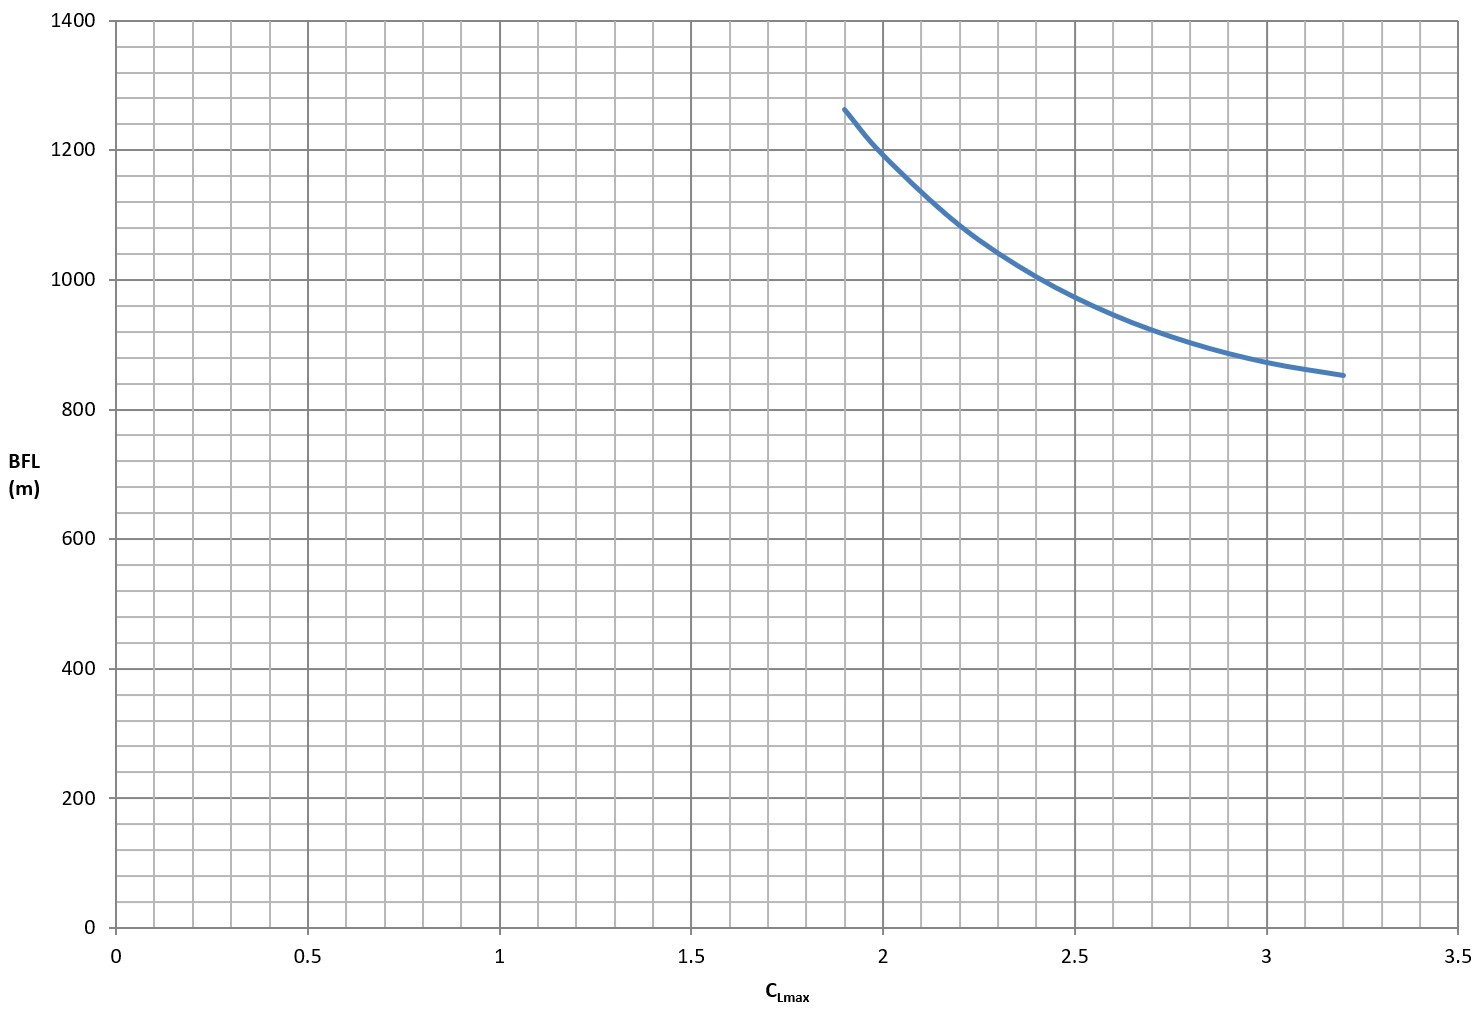
\includegraphics[width=1.1\textwidth]{pictures/BFL_CL.jpg}
\end{figure}

\section{Group Work Evaluation}
Overall, the design team has worked exceptionally well together throughout the course of this project. Each member of the team had clear assignments and objectives and was supported in the completion of these objectives by the rest of the team. As a whole, the group worked together to achieve most design objectives, with each aspect of design having a primary, which gave the added bonus of leadership experience to all group members throughout the project. In addition, the group members regularly communicated with one another and secured their files via Microsoft Teams. In addition to Teams, all documents were version controlled, which meant that all team members could see who made modifications, and where, and if necessary, revert to a previous version of the document with the click of a button.  
\section{Conclusions}
To summarise, the design team successfully designed an aircraft that achieves the original objectives. The aircraft that has been designed is capable of:
\begin{enumerate}
    \item Transporting specialty cargo and personnel, 
    \item Operating from short field lengths and,
    \item Acting as a short-range transport aircraft.
\end{enumerate}
While the aircraft's performance is generally very good, the author recommends further improving the value for the Balanced Field length (just over 1000m), which will make the aircraft even more suitable for operating in and out of potentially hazardous environments. But other than that, the aircraft is able to compete with existing aircraft on the market by being lightweight (84kN) but having a large transport capacity (24kN), making it comparatively much cheaper to operate than other alternatives that already are in circulation. Most importantly, not only does the design meet the objectives, but it is also stable (as seen in Figures 3.1 and 4.1) as the aircraft is perfectly balanced. It also meets all necessary certification requirements as laid out in EASA Part-25 for large aeroplanes. Overall all the design choices are suitable for the aircraft that was designed. 
This was ultimately achieved by a design team that collaborated effectively, where all team members had the common goal of working towards creating an aircraft that has the potential to have a very positive impact on our world.

\addcontentsline{toc}{section}{6 References}
\printbibliography
\end{document}